\section{Modelling \& Simulation}

\subsection{Single Compressor}
\begin{frame}{Compressor Model}
  What model is used for the compressor?\\
  Where does it come from?\\
  What are the significant non-linearities?\\
  Inputs/outputs/states
\end{frame}

\begin{frame}{Surge Distance}
  What is surge distance and why does it matter?\\
  How do we model it?\\
\end{frame}

\subsection{Compressor Systems}

\begin{frame}{Parallel System}
  Overview of system\\
  Assumptions made\\
  Inputs/outputs/states
\end{frame}

\begin{frame}{Serial System}
  Overview of system\\
  Assumptions made\\
  Inputs/outputs/states
\end{frame}

\subsection{Simulation}
\begin{frame}{Simulation}
  Simulink parameters\\
  C++ parameters
\end{frame}


\begin{frame}{Models}
  \begin{figure}[H]
    \centering
    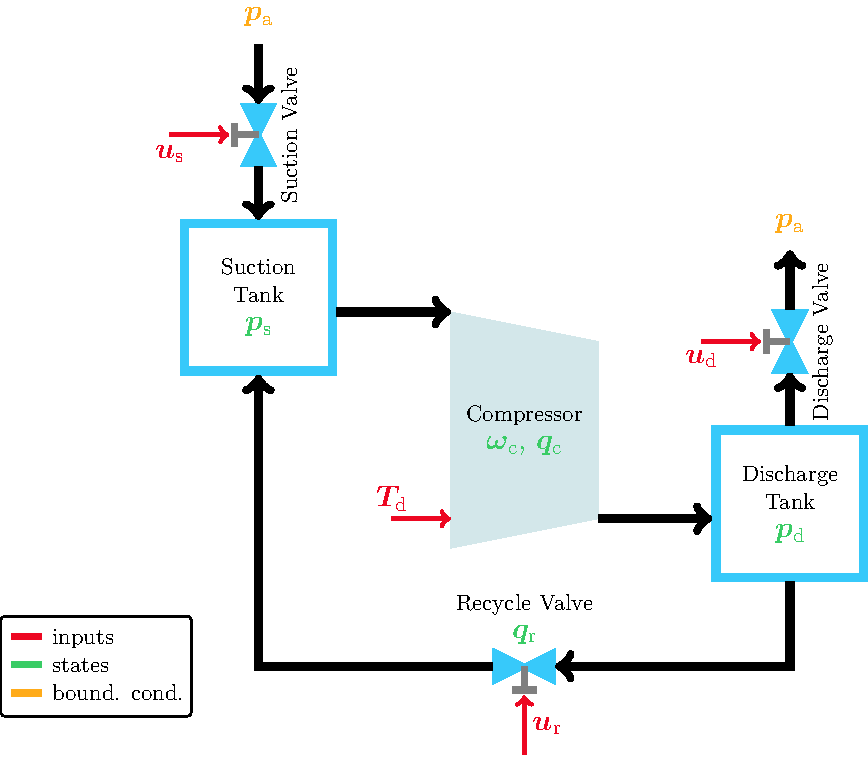
\includegraphics[width=.5\linewidth]{figures/compressor.pdf}
  \end{figure}
\end{frame}

\begin{frame}{Models}
  \begin{figure}[H]
    \centering
    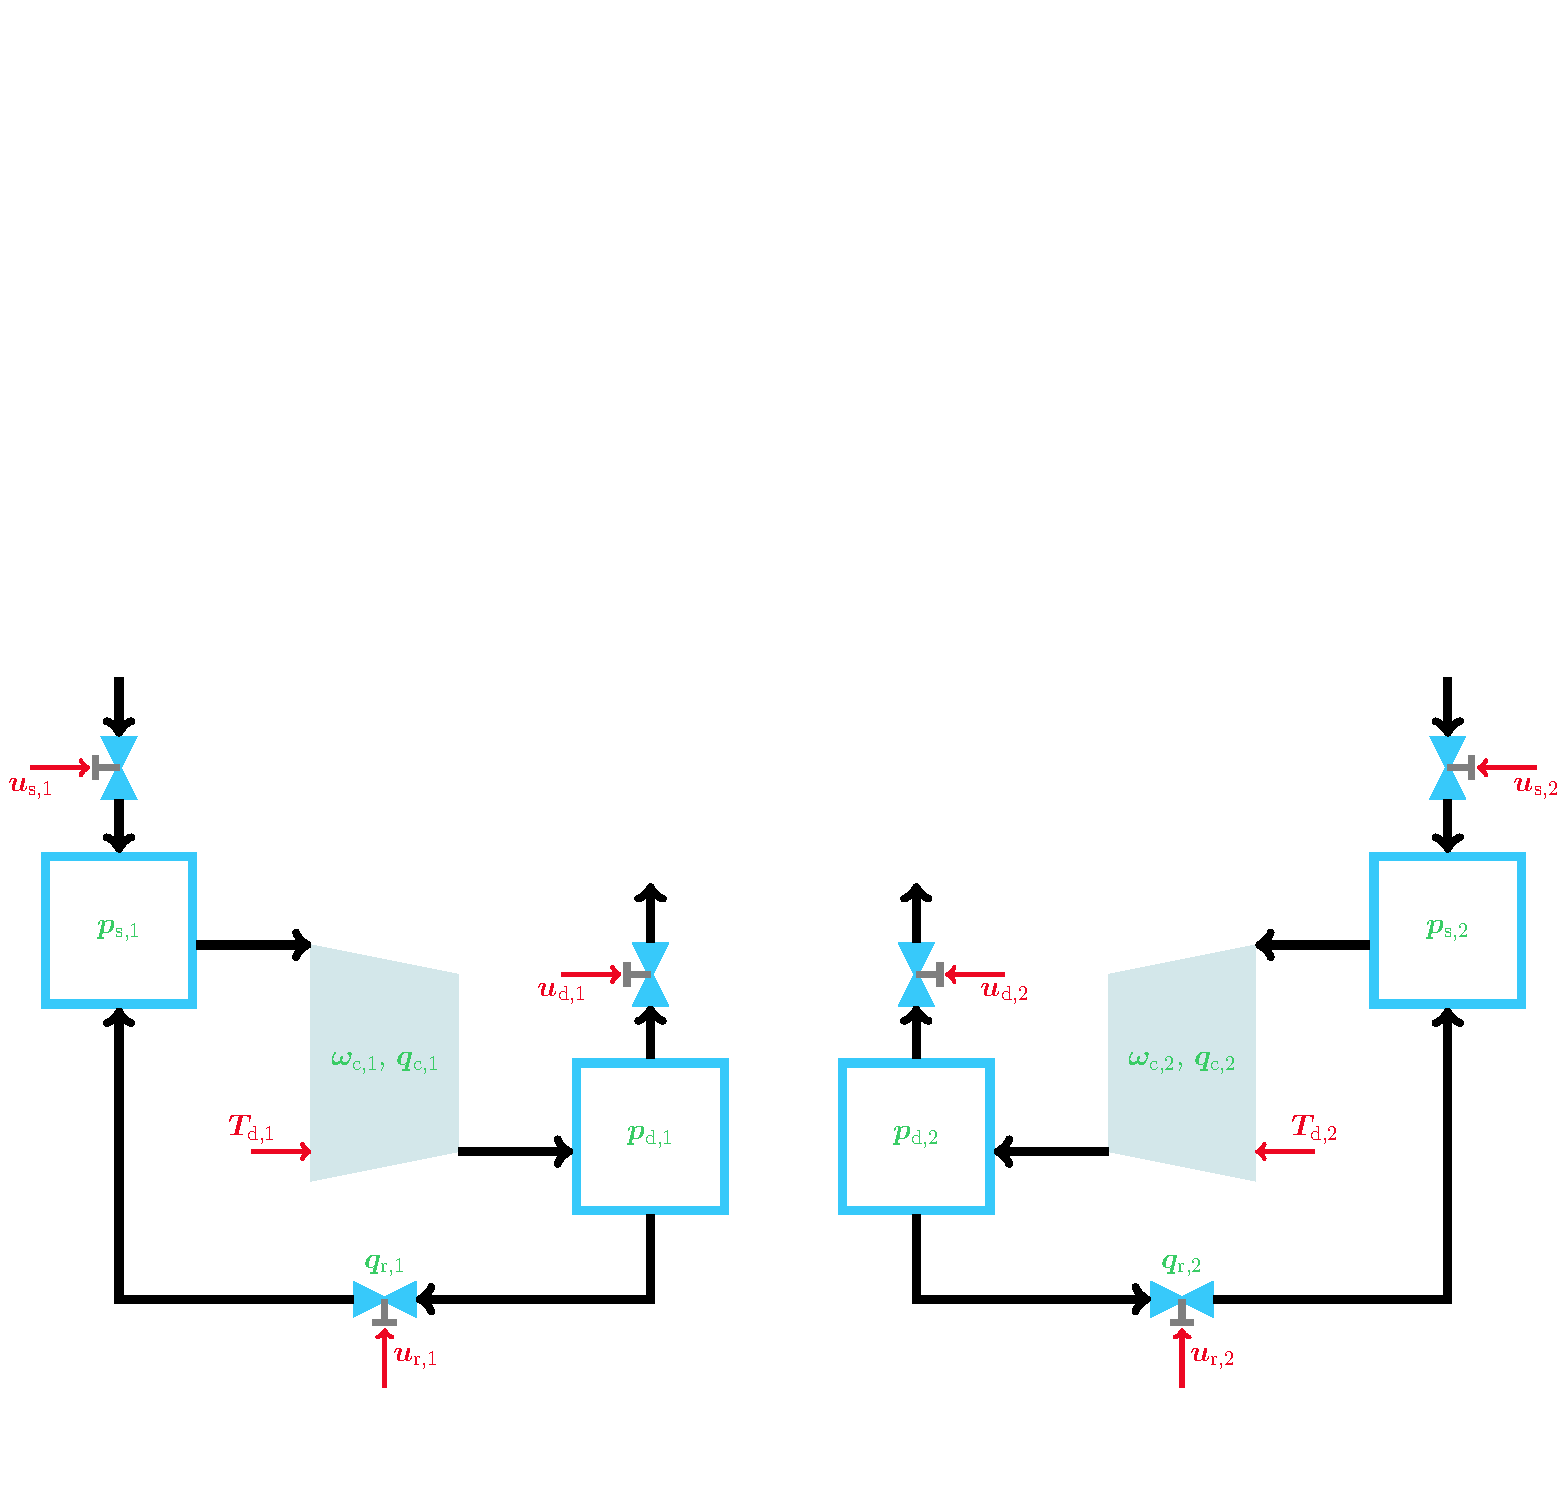
\includegraphics[width=.8\linewidth]{figures/parallelcompressor.pdf}
  \end{figure}
\end{frame}

\begin{frame}{Models}
  \begin{figure}[H]
    \centering
    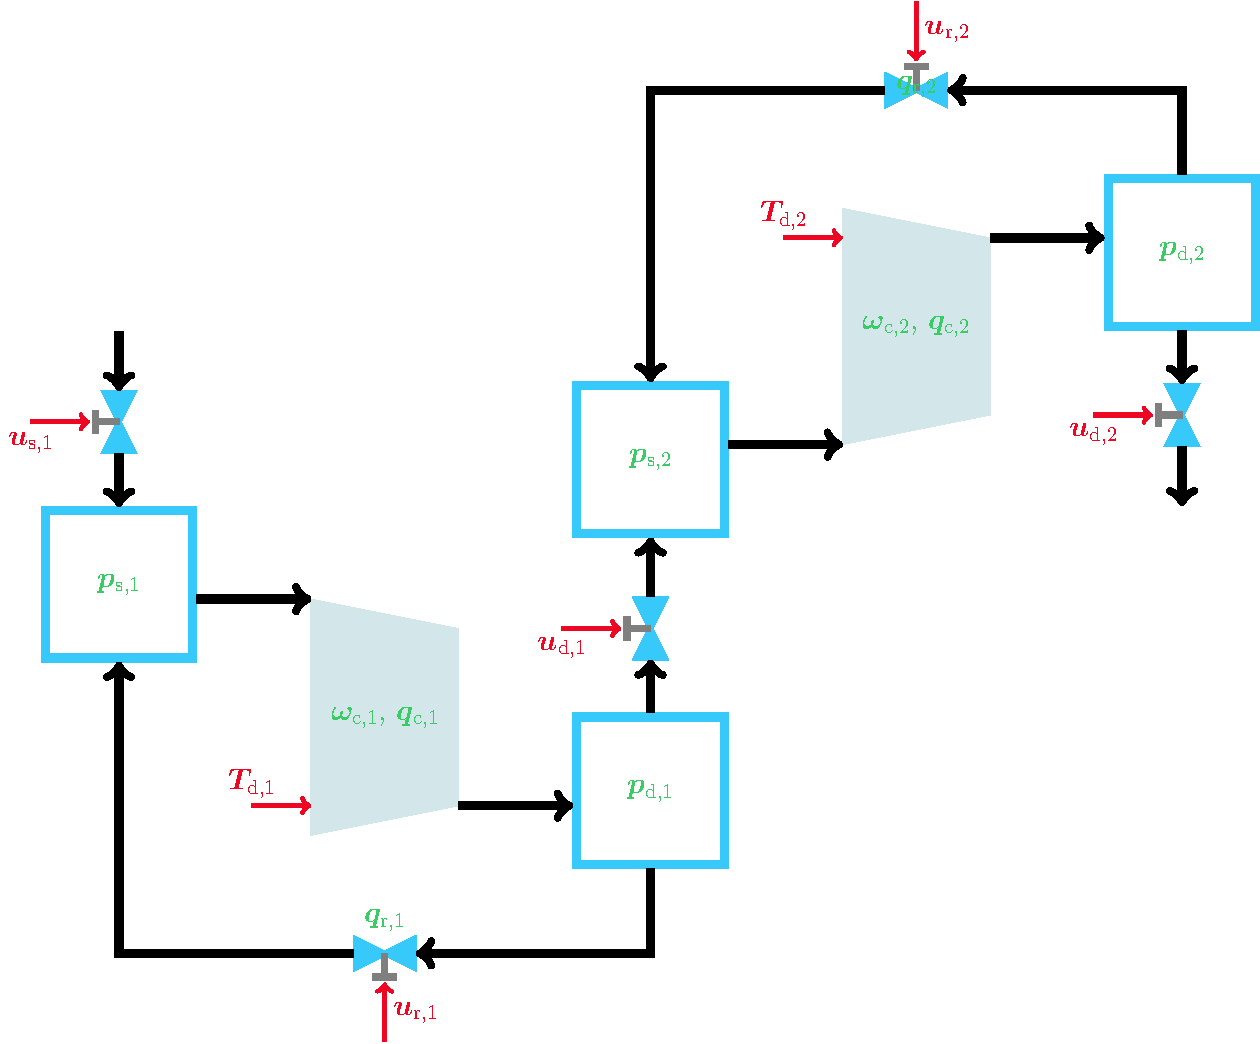
\includegraphics[width=.5\linewidth]{figures/serialcompressor.pdf}
  \end{figure}
\end{frame}

\begin{frame}{Models}
  \begin{figure}[H]
    \centering
    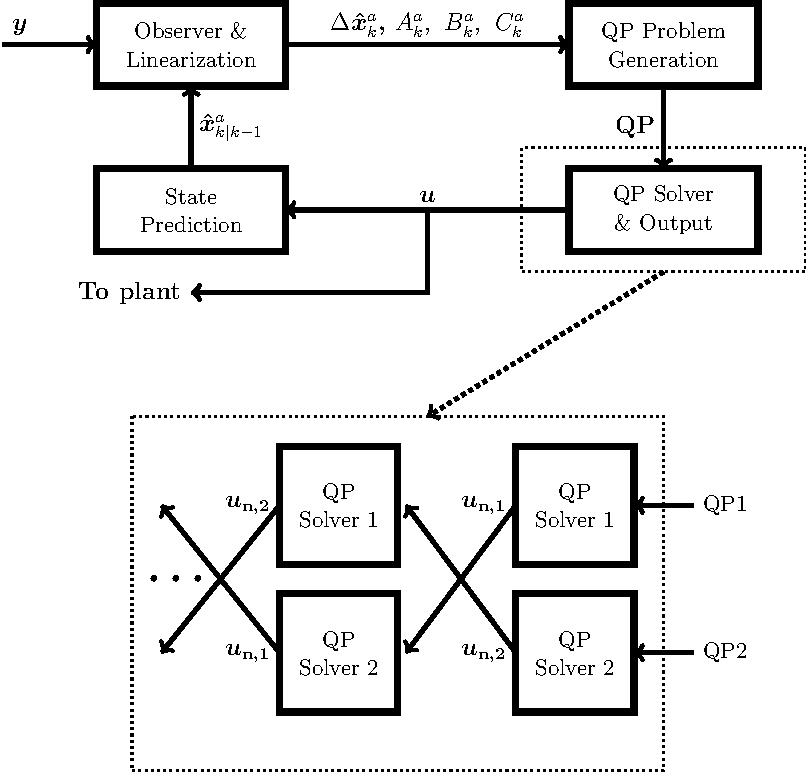
\includegraphics[width=.5\linewidth]{figures/algorithm.pdf}
  \end{figure}
\end{frame}
